\begin{problem}{\#1 (15 points)}
    Use the pumping lemma to show that this language is nonregular:
    \begin{align*}
        \{a^nb^na^n\} &= \{aba,aabbaa,aaabbbaaa,\ldots\}\\
        \{a^nba^n\} &= \{aba,aabaa,aaabaaa,\ldots\}\\
        \{a^nb^{2n} &= \{abb,aabbbb,aaabbbbbb,\ldots\}
    \end{align*}
\end{problem}
\begin{solution}
    \begin{enumerate}
        \item First we assume that $L$ is regular and $n$ is the number of states.\\
        Let $w = a^nb^na^n$. Thus $|w| = 3n \geq n$.\\
        By pumping lemma, let $w = xyz$, where $|xy|\leq n$.\\
        Let $x=a^p,y=a^q,z=a^rb^na^n$, where $p+q+r=n, p\neq 0, q \neq 0, r\neq 0$.\\
        Let $k=2$. Then $xy^2z=a^pa^{2q}a^rb^na^n$.\\
        The number of $a$'s is :$\left( p+2q+r \right)+n=\left( p+q+r \right)+q+n = 2n+q$\\
        Hence, $xy^2z=a^{n+q}b^na^n$. Since $q\neq 0, xy^2z$ is not of the form $a^nb^na^n$.\\
        Thus, $xy^2z$ is not in $L$ making $L$ not regular.
        \item First we assume that $L$ is regular and $n$ is the number of states.\\
        Let $w = a^nba^n$. Thus $|w| = 2n+1 \geq n$.\\
        By pumping lemma, let $w=xyz$, where $|xy|\leq n$.\\
        Let $x=a^p,y=a^q,z=a^rba^n$, where $p+q+r=n,p\neq 0,q\neq 0, r\neq 0$.\\
        Let $k=2$. Then $xy^2z=a^pa^{2q}a^rba^n$.\\
        The number of $a$'s is: $\left( q+2q+r \right)+n=\left( p+q+r \right)+q+n = 2n+q$\\
        Hence, $xy^2z=a^{n+q}ba^n$. Since $q\neq 0, xy^2z$ is not of the form $a^nba^n$.\\
        Thus $xy^2z$ is not in $L$ making $L$ not regular. 
        \item First we assume that $L$ is regular and $n$ is the number of states.\\
        Let $w = a^nb^{2n}$. Thus $|w| = 3n \geq n$.\\
        By pumping lemma, let $w=xyz$, where $|xy|\leq n$.\\
        Let $x=a^p,y=a^q,z=a^rb^{2n}$, where $p+q+r=n,p\neq 0,q\neq 0, r\neq 0$.\\
        Let $k=2$. Then $xy^2z=a^pa^{2q}a^rb^{2n}$.\\
        The number of $a$'s is: $\left( q+2q+r \right)=\left( p+q+r \right)+q = n+q$\\
        Hence, $xy^2z=a^{n+q}b^{2n}$. Since $q\neq 0, xy^2z$ is not of the form $a^nb^{2n}$.\\
        Thus $xy^2z$ is not in $L$ making $L$ not regular.
    \end{enumerate}
\end{solution}

\begin{problem}{\#2 (10 points)}
    By using blue paint, determine which of the following FA's accept any words:
    \begin{enumerate}[label=\alph*)]
        \item 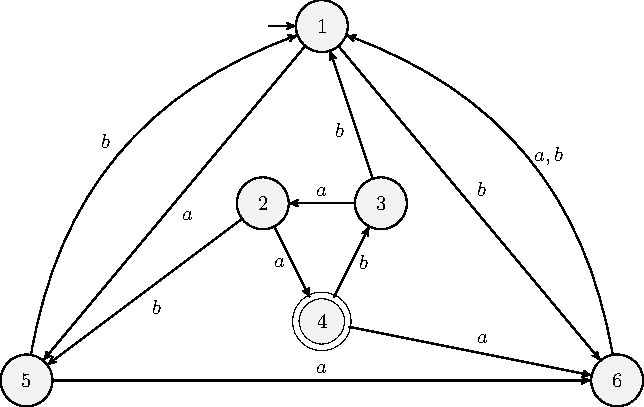
\includegraphics[width=0.7\linewidth]{figures/questions/2a.pdf}
        \item 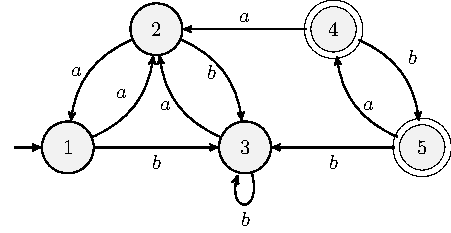
\includegraphics[width=0.6\linewidth]{figures/questions/2b.pdf}
    \end{enumerate}
\end{problem}
\begin{solution}
    \begin{enumerate}
        \item 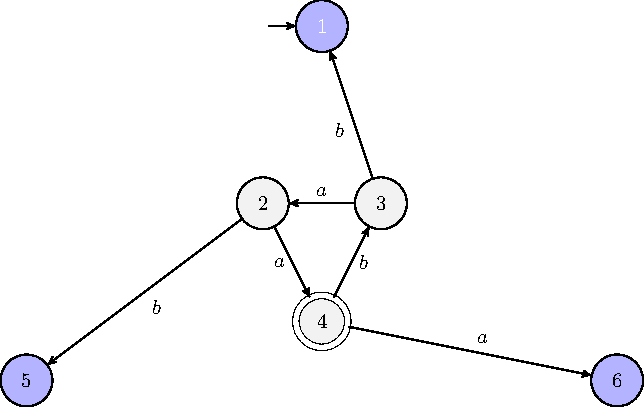
\includegraphics[width=0.7\linewidth]{figures/answers/2a.pdf}
        \item 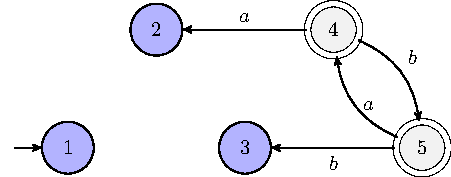
\includegraphics[width=0.6\linewidth]{figures/answers/2b.pdf}
    \end{enumerate}
\end{solution}

\begin{problem}{\#3 (18 points)}
    Describe the language generated by the following context free grammar (CFG) in English and regular expressions:
    \begin{enumerate}[label=\alph*)]
        \item $S \to SS$\\
        $S \to ZZZ$\\
        $Z \to bZ$\\
        $Z \to Zb$\\
        $Z \to a$
        \item $S \to aS$\\
        $S \to bb$
        \item $S \to XYX$\\
        $X \to aX$\\
        $X \to bX$\\
        $X \to \Lambda$\\
        $Y \to bbb$
    \end{enumerate}
\end{problem}
\begin{solution}
    \begin{enumerate}[label=\alph*)]
        \item This CFG can be described as any number of $b$'s with a multiple of 3 $a$'s.\\
        Regular Expression: $\left(b^*ab^*ab^*ab^*\right)^*$ 
        \item This CFG can be described as any number of $a$'s followed by two $b$'s.\\
        Regular Expression: $a^*bb$
        \item This CFG can be described as any string of $a$'s and $b$'s containing the string $bbb$.\\
        Regular Expression: $(a+b)^*bbb(a+b)^*$
    \end{enumerate}
\end{solution}

\begin{problem}{\#4 (15 points)}
    Find CFG for the following languages over the alphabet $\Sigma = \{a,b\}$:
    \begin{enumerate}[label=\alph*)]
        \item All words that have different first and last letters.
        \item All words in which the letter $b$ is never tripled.
        \item All words that do not have substring $ab$.
    \end{enumerate}
\end{problem}
\begin{solution}
    \begin{enumerate}[label=\alph*)]
        \item $S \to aXb \mid bXa$\\
        $X \to aX \mid bX \mid a \mid b \mid \Lambda$
        \item $S \to \Lambda \mid b \mid bb \mid Sa \mid aS \mid Sab \mid Sabb$
        \item $S \to \Lambda \mid bS \mid bX \mid X$\\
        $X \to aX \mid \Lambda$
    \end{enumerate}
\end{solution}

\begin{problem}{\#5 (10 points)}
    Show that the CFG below is ambiguous by finding a word with two distinct syntax trees.
    Show both syntax trees.
    \begin{enumerate}[label=\alph*)]
        \item $S \to Sbb$\\
        $S \to Sbbb$\\
        $S \to b$\\
        \item $S \to AA$\\
        $A \to AAA|a|bA|Ab$
    \end{enumerate}
\end{problem}
\begin{solution}
    \begin{enumerate}
        \item The CFG is ambiguous because the word $bbbbbb$ can follow:\\
        \begin{table}[h]
            \centering\begin{tabular}{l|l|l}
                \textbf{Rule} & \textbf{Application} & \textbf{Result}\\
                \hline
                Start $\to$ S & Start & S\\
                S $\to$ Sbbb & \textbf{S} & \textbf{Sbbb}\\
                S $\to$ Sbb & \textbf{S}bbb & \textbf{Sbb}bbb\\
                S $\to$ b & \textbf{S}bbbbb & \textbf{b}bbbbb\\
                \hline
                Start $\to$ S & Start & S\\
                S $\to$ Sbb & \textbf{S} & \textbf{Sbb}\\
                S $\to$ Sbbb & \textbf{S}bb & \textbf{Sbbb}bb\\
                S $\to$ b & \textbf{S}bbbbb & \textbf{b}bbbbb
            \end{tabular}
            % \caption{}
            \label{tb:q5a}
        \end{table}
        \item The CFG is ambiguous because the word $aba$ can follow:\\
        \begin{table}[h]
            \centering\begin{tabular}{l|l|l}
                \textbf{Rule} & \textbf{Application} & \textbf{Result}\\
                \hline
                Start $\to$ S & Start & S\\
                S $\to$ AA & \textbf{S} & \textbf{AA}\\
                A $\to$ Ab & \textbf{A}A & \textbf{Ab}A\\
                A $\to$ a & \textbf{A}bA & \textbf{a}bA\\
                A $\to$ a & ab\textbf{A} & ab\textbf{a}\\
                \hline
                Start $\to$ S & Start & S\\
                S $\to$ AA & \textbf{S} & \textbf{AA}\\
                A $\to$ a & \textbf{A}A & \textbf{a}A\\
                A $\to$ bA & a\textbf{A} & a\textbf{bA}\\
                A $\to$ a & ab\textbf{a} & ab\textbf{a}
            \end{tabular}
        \end{table}
    \end{enumerate}
\end{solution}
